\documentclass{article}
\usepackage[paperwidth=7.2in,paperheight=2.25in,margin=0.05in]{geometry}
\usepackage{tikz}
\usetikzlibrary{arrows.meta,positioning,fit}
\pagestyle{empty}
\begin{document}
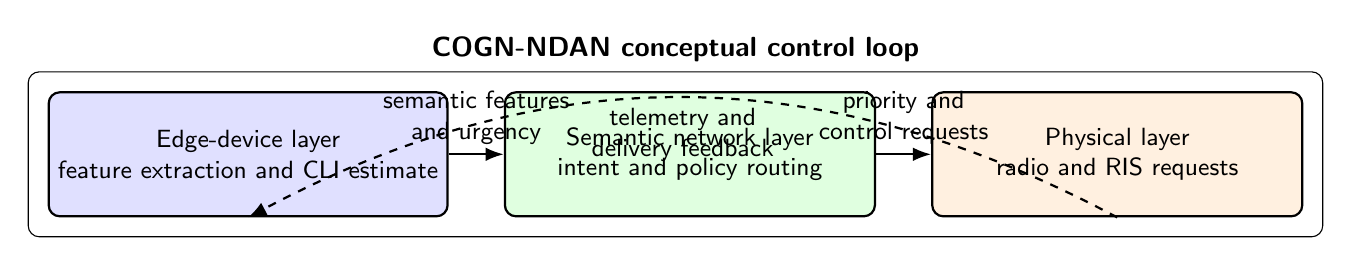
\begin{tikzpicture}[font=\sffamily\small, >=Latex, node distance=5mm and 7mm,
  layer/.style={draw, rounded corners, align=center, minimum width=1.85in, minimum height=0.62in, fill=#1!12, thick},
  flow/.style={->, thick}, feedback/.style={->, dashed, thick}]
  \node[layer=blue] (edge) {Edge-device layer\\feature extraction and CLI estimate};
  \node[layer=green, right=of edge] (semantic) {Semantic network layer\\intent and policy routing};
  \node[layer=orange, right=of semantic] (physical) {Physical layer\\radio and RIS requests};
  \draw[flow] (edge) -- node[above, align=center] {semantic features\\and urgency} (semantic);
  \draw[flow] (semantic) -- node[above, align=center] {priority and\\control requests} (physical);
  \draw[feedback] (physical.south) to[bend right=28] node[below, align=center] {telemetry and\\delivery feedback} (edge.south);
  \node[draw, rounded corners, fit=(edge)(semantic)(physical), inner sep=7pt, label={[font=\bfseries\sffamily]above:COGN-NDAN conceptual control loop}] {};
\end{tikzpicture}
\end{document}
